\documentclass[12pt,a4paper]{article}
\usepackage[utf8]{vietnam}
\usepackage{amsmath,amssymb}
\usepackage{tabularx}
\usepackage{tikz}
\usetikzlibrary{calc,angles,quotes,arrows.meta}
\usepackage{xcolor}
\usepackage{enumitem}
\usepackage{fancyhdr}
\usepackage[top=1.2cm, bottom=1.2cm, left=1.5cm, right=1.5cm]{geometry}
\usepackage[dethi]{ex_test}
\SAOPTN{widthSA=2.6,heightSA=0.62}

\setlength{\headheight}{15pt}
\setlength{\parskip}{0pt}

% Dòng kẻ chấm mờ chuẩn viết tay
\newcommand{\dongke}[1]{%
  \begingroup%
  \setlength{\parskip}{0pt}%
  \baselineskip=18.5pt%
  \vspace{1.0mm}%
  \foreach \i in {1,...,#1}{%
    \noindent{\color{gray!60}\dotfill}\par%
  }%
  \vspace{0.6mm}%
  \endgroup%
}

\pagestyle{fancy}
\fancyhf{}
\rhead{\textit{Môn Toán 7 -- Đề số 5}}
\lhead{\textit{Bộ đề ôn tập Giữa học kì I}}
\cfoot{\thepage}

\begin{document}

% --- KHUNG TIÊU ĐỀ ĐỀ THI ---
\noindent
\begin{tabularx}{\linewidth}{X r}
\textbf{TRƯỜNG THCS: \dotfill} & \textbf{ĐỀ KIỂM TRA ĐỊNH KỲ GIỮA HỌC KỲ I} \\
\textbf{Họ và tên: \dotfill} & \textbf{NĂM HỌC 2026 -- 2027} \\
\textbf{Lớp: \dotfill \quad SBD: \dotfill} & \textbf{Môn: TOÁN 7} \\
& \textit{Thời gian làm bài: 90 phút (không kể thời gian phát đề)}
\end{tabularx}

\vspace{1.5mm}
\noindent
\begin{tabularx}{\linewidth}{|p{3.5cm}|X|}
\hline
\centering\textbf{Điểm số} & \centering\textbf{Lời nhận xét của thầy cô giáo} \tabularnewline
\rule{0pt}{1.6cm} & \\
\hline
\end{tabularx}

\vspace{2.5mm}
\begin{center}
\textbf{\large ĐỀ SỐ 5}
\end{center}

\noindent\textbf{\large PHẦN I. CÂU TRẮC NGHIỆM NHIỀU PHƯƠNG ÁN LỰA CHỌN (3,0 điểm)}

\textit{Thí sinh trả lời từ câu 1 đến câu 12. Mỗi câu hỏi chỉ chọn một phương án đúng nhất và ghi vào bảng đáp án.}

\vspace{1mm}
\begin{ex}
Cho các số sau: $\dfrac{5}{4}; 3\dfrac{2}{5}; \dfrac{-2}{7}; \dfrac{0}{3}; \dfrac{-3}{0}; \dfrac{8}{8}; 0{,}625$. Hãy cho biết số nào không phải là số hữu tỉ?
\choice
{\True $\dfrac{-3}{0}$}
{$0{,}625$}
{$\dfrac{-2}{7}$}
{$3\dfrac{2}{5}$}
\end{ex}

\begin{ex}
Kết quả của phép tính $(2{,}023)^0$ là:
\choice
{$2$}
{$0$}
{$2{,}023$}
{\True $1$}
\end{ex}

\begin{ex}
Với $x, y, z$ là ba số hữu tỉ bất kì, sau khi bỏ ngoặc ta được $-(x - y + z)$ bằng:
\choice
{\True $-x + y - z$}
{$-x - y - z$}
{$x + y - z$}
{$x + y + z$}
\end{ex}

\begin{ex}
\immini{
Cho hình vẽ sau, nếu $a \parallel b$ thì:
\choice
{$\widehat{M}_1 = \widehat{N}_2$}
{$\widehat{M}_3 = \widehat{N}_4$}
{\True $\widehat{M}_4 = \widehat{N}_4$}
{$\widehat{M}_4 = \widehat{N}_3$}
}{
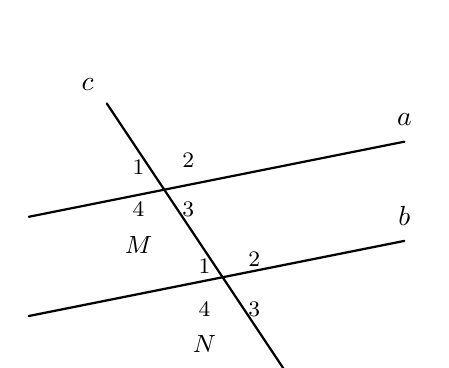
\begin{tikzpicture}[scale=0.9, line cap=round, line join=round]
  \draw[thick] (-2.5, 0.7) -- (2.8, 1.76) node[above=2pt] {$a$};
  \draw[thick] (-2.5, -0.7) -- (2.8, 0.36) node[above=2pt] {$b$};
  \draw[thick] (-1.4, 2.3) node[above left=1pt] {$c$} -- (1.2, -1.6);
  \node[font=\footnotesize] at (-0.95, 1.4) {$1$};
  \node[font=\footnotesize] at (-0.25, 1.5) {$2$};
  \node[font=\footnotesize] at (-0.25, 0.8) {$3$};
  \node[font=\footnotesize] at (-0.95, 0.8) {$4$};
  \node[font=\small, below=6pt] at (-0.95, 0.8) {$M$};
  \node[font=\footnotesize] at (-0.02, 0.0) {$1$};
  \node[font=\footnotesize] at (0.68, 0.1) {$2$};
  \node[font=\footnotesize] at (0.68, -0.6) {$3$};
  \node[font=\footnotesize] at (-0.02, -0.6) {$4$};
  \node[font=\small, below=6pt] at (-0.02, -0.6) {$N$};
\end{tikzpicture}
}
\end{ex}

\begin{ex}
Cho biểu thức $\left(\dfrac{1}{2} - \dfrac{1}{3}\right) + \left(\dfrac{1}{2} - \dfrac{1}{3}\right) - \left(\dfrac{1}{2} + \dfrac{2}{3}\right)$. Khi bỏ dấu ngoặc, ta được biểu thức:
\choice
{$\dfrac{1}{2} - \dfrac{1}{3} + \dfrac{1}{2} - \dfrac{1}{3} - \dfrac{1}{2} + \dfrac{2}{3}$}
{$\dfrac{1}{2} - \dfrac{1}{3} + \dfrac{1}{2} - \dfrac{1}{3} + \dfrac{1}{2} - \dfrac{2}{3}$}
{$\dfrac{1}{2} - \dfrac{1}{3} + \dfrac{1}{2} + \dfrac{1}{3} - \dfrac{1}{2} - \dfrac{2}{3}$}
{\True $\dfrac{1}{2} - \dfrac{1}{3} + \dfrac{1}{2} - \dfrac{1}{3} - \dfrac{1}{2} - \dfrac{2}{3}$}
\end{ex}

\begin{ex}
\immini{
Cho $a \parallel b$, số đo góc $x$ trên hình vẽ bằng:
\choice
{\True $115^\circ$}
{$90^\circ$}
{$65^\circ$}
{$0^\circ$}
}{
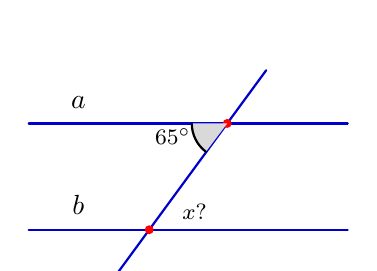
\begin{tikzpicture}[scale=0.9, line cap=round, line join=round]
  \coordinate (A) at (0.8, 1.3);
  \coordinate (B) at (-0.3, -0.2);
  \draw[thick, blue!80!black] (-2, 1.3) -- (2.5, 1.3);
  \node[above=2pt] at (-1.3, 1.3) {$a$};
  \draw[thick, blue!80!black] (-2, -0.2) -- (2.5, -0.2);
  \node[above=2pt] at (-1.3, -0.2) {$b$};
  \draw[thick, blue!80!black] (-0.85, -0.95) -- (1.35, 2.05);
  \fill[red] (A) circle (1.8pt);
  \fill[red] (B) circle (1.8pt);
  \fill[gray!30] (A) -- ++(180:0.5) arc (180:233:0.5) -- cycle;
  \draw[thick] (A) ++(180:0.5) arc (180:233:0.5);
  \node[font=\footnotesize, left=2pt] at ($(A)+(-0.3,-0.18)$) {$65^\circ$};
  \node[font=\footnotesize, right=2pt] at ($(B)+(0.25,0.25)$) {$x?$};
\end{tikzpicture}
}
\end{ex}

\begin{ex}
Căn bậc hai số học của $9$ là:
\choice
{$-3$}
{\True $3$}
{$\pm 3$}
{$81$}
\end{ex}

\begin{ex}
Trong các câu sau, câu nào không phải là định lí?
\choice
{Tổng ba góc trong một tam giác bằng $180^\circ$}
{Hai đường thẳng phân biệt vuông góc với cùng một đường thẳng thì song song với nhau}
{Hai góc đối đỉnh thì bằng nhau}
{\True $2 + 2 = 5$}
\end{ex}

\begin{ex}
Chọn đáp án đúng. Trong hình vuông:
\choice
{Hai đường chéo bằng nhau}
{\True Cả 3 khẳng định còn lại đều đúng}
{Bốn cạnh bằng nhau}
{Bốn góc ở các đỉnh là góc vuông}
\end{ex}

\begin{ex}
Lan viết các số La Mã như sau: XIII, XIX, VXI, XXIV. Lan viết sai số La Mã nào?
\choice
{XIII}
{XIX}
{\True VXI}
{XXIV}
\end{ex}

\begin{ex}
Cho hai tam giác $ABC$ và $DEF$ có $AB = EF, BC = FD, AC = ED$. Khi đó:
\choice
{$\Delta ABC = \Delta DEF$}
{$\Delta ABC = \Delta FDE$}
{$\Delta ABC = \Delta DFE$}
{\True $\Delta ABC = \Delta EFD$}
\end{ex}

\begin{ex}
Khẳng định nào sau đây đúng?
\choice
{$(-2)^8 = -2^8$}
{$\left(-\dfrac{2}{3}\right)^3 = \dfrac{6}{9}$}
{$[(-2)^3]^2 = -2^5$}
{\True $\left(-\dfrac{1}{2}\right)^4 = \dfrac{1}{16}$}
\end{ex}


\vspace{1mm}
\noindent\textbf{BẢNG TRẢ LỜI TRẮC NGHIỆM PHẦN I:}
\begin{center}
\begin{tabular}{|c|c|c|c|c|c|c|c|c|c|c|c|c|}
\hline
\textbf{Câu} & \textbf{1} & \textbf{2} & \textbf{3} & \textbf{4} & \textbf{5} & \textbf{6} & \textbf{7} & \textbf{8} & \textbf{9} & \textbf{10} & \textbf{11} & \textbf{12} \\
\hline
\textbf{Chọn} & \rule{0pt}{0.65cm} & & & & & & & & & & & \\
\hline
\end{tabular}
\end{center}
\vspace{2mm}

\setcounter{ex}{0}
\noindent\textbf{\large PHẦN II. CÂU TRẮC NGHIỆM ĐÚNG SAI (2,0 điểm)}

\textit{Thí sinh trả lời câu 1 và câu 2. Trong mỗi ý a), b), c), d) ở mỗi câu, thí sinh chọn đúng hoặc sai.}

\vspace{1mm}
\begin{ex}
\immini{
Cho hai đường thẳng cắt nhau tại điểm $O$ tạo thành bốn góc $\widehat{O}_1, \widehat{O}_2, \widehat{O}_3, \widehat{O}_4$. Xét tính đúng sai của các mệnh đề sau:
\choiceTF
{\True Hai góc $\widehat{O}_1$ và $\widehat{O}_3$ là hai góc đối đỉnh}
{\True Hai góc $\widehat{O}_2$ và $\widehat{O}_3$ là hai góc kề bù}
{Hai góc $\widehat{O}_1$ và $\widehat{O}_3$ có tổng số đo bằng $180^\circ$}
{Hai góc $\widehat{O}_2$ và $\widehat{O}_4$ là hai góc đối đỉnh nên có số đo bằng $180^\circ$}
}{
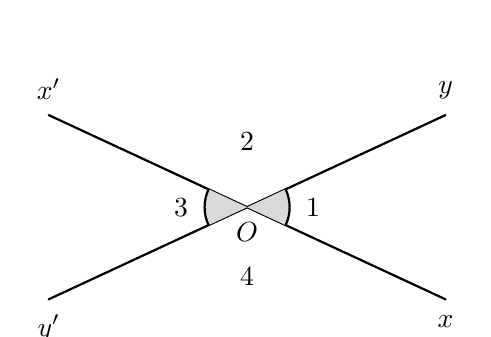
\begin{tikzpicture}[scale=0.9, line cap=round, line join=round]
  \coordinate (O) at (0,0);
  \draw[thick] (-2.8,1.3) node[above=2pt] {$x'$} -- (2.8,-1.3) node[below=2pt] {$x$};
  \draw[thick] (-2.8,-1.3) node[below=2pt] {$y'$} -- (2.8,1.3) node[above=2pt] {$y$};
  \fill[gray!30] (O) -- (25:0.6) arc (25:-25:0.6) -- cycle;
  \draw[thick] (25:0.6) arc (25:-25:0.6);
  \fill[gray!30] (O) -- (155:0.6) arc (155:205:0.6) -- cycle;
  \draw[thick] (155:0.6) arc (155:205:0.6);
  \node[right=5pt] at (0.5,0) {$1$};
  \node[above=4pt] at (0,0.5) {$2$};
  \node[left=5pt] at (-0.5,0) {$3$};
  \node[below=8pt] at (0,-0.4) {$4$};
  \node[below=2pt] at (O) {$O$};
\end{tikzpicture}
}
\end{ex}

\begin{ex}
\immini{
Cho $\widehat{xOy} = 70^\circ$. Trên tia $Ox$ lấy điểm $A$. Kẻ tia $Az$ sao cho $\widehat{xAz} = 70^\circ$. Trên tia $Az$ lấy điểm $B$, kẻ tia $Bt$ cắt $Oy$ tại $C$ sao cho $\widehat{CBA} = 110^\circ$. Xét tính đúng sai của các mệnh đề sau:
\choiceTF
{\True $\widehat{ABC}$ và $\widehat{CBz}$ là hai góc kề bù}
{\True $\widehat{CBz} = 70^\circ$}
{\True $Oy$ song song với $Az$}
{$\widehat{BCO} = 110^\circ$}
}{
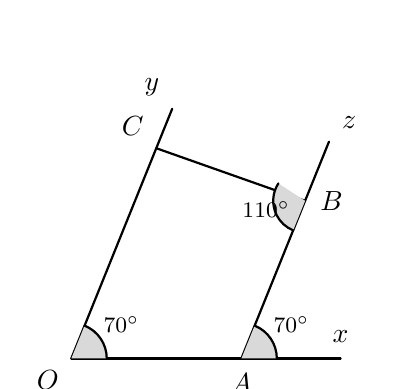
\begin{tikzpicture}[scale=0.9, line cap=round, line join=round]
  \coordinate (O) at (0,0);
  \coordinate (A) at (2.4,0);
  \coordinate (B) at ($(A)+(68:2.4)$);
  \coordinate (C) at ($(O)+(68:3.2)$);
  \draw[thick] (O) -- (3.8,0) node[above=2pt] {$x$};
  \draw[thick] (O) -- ($(O)+(68:3.8)$) node[above left=1pt] {$y$};
  \draw[thick] (A) -- ($(A)+(68:3.3)$) node[above right=1pt] {$z$};
  \draw[thick] (C) -- (B);
  \fill[gray!30] (O) -- (0.5,0) arc (0:68:0.5) -- cycle;
  \draw[thick] (0.5,0) arc (0:68:0.5);
  \node[font=\footnotesize] at (34:0.85) {$70^\circ$};
  \fill[gray!30] (A) -- ++(0:0.5) arc (0:68:0.5) -- cycle;
  \draw[thick] (A) ++(0:0.5) arc (0:68:0.5);
  \node[font=\footnotesize] at ($(A)+(34:0.85)$) {$70^\circ$};
  \fill[gray!30] (B) -- ++(147:0.45) arc (147:248:0.45) -- cycle;
  \draw[thick] (B) ++(147:0.45) arc (147:248:0.45);
  \node[font=\footnotesize] at ($(B)+(-0.55,-0.12)$) {$110^\circ$};
  \node[below left=1pt] at (O) {$O$};
  \node[below=2pt] at (A) {$A$};
  \node[right=2pt] at (B) {$B$};
  \node[above left=1pt] at (C) {$C$};
\end{tikzpicture}
}
\end{ex}


\noindent\textbf{BẢNG TRẢ LỜI PHẦN II:}
\begin{center}
\begin{tabular}{|c|c|c|c|c||c|c|c|c|c|}
\hline
\textbf{Câu 1} & \textbf{a)} & \textbf{b)} & \textbf{c)} & \textbf{d)} & \textbf{Câu 2} & \textbf{a)} & \textbf{b)} & \textbf{c)} & \textbf{d)} \\
\hline
\textbf{Đ/S} & \rule{0pt}{0.6cm} & & & & \textbf{Đ/S} & & & & \\
\hline
\end{tabular}
\end{center}
\vspace{2mm}

\setcounter{ex}{0}
\noindent\textbf{\large PHẦN III. CÂU HỎI TRẢ LỜI NGẮN (1,0 điểm)}

\textit{Thí sinh trả lời câu 1 và câu 2. Điền kết quả vào ô trống.}

\vspace{1mm}
\begin{ex}
Tìm số tự nhiên $x$, biết: $2^{x+3} + 2^x = 144$. \shortans{$x = 4$}
\end{ex}

\begin{ex}
Cho hai đường thẳng song song $a$ và $b$. Đường thẳng $c$ cắt $a$ và $b$ lần lượt tại hai điểm $A$ và $B$. Biết góc $\widehat{A}_1$ và góc $\widehat{B}_1$ là hai góc trong cùng phía, trong đó $\widehat{A}_1 = 65^\circ$. Tính số đo góc $\widehat{B}_1$. \shortans{$\widehat{B}_1 = 115^\circ$}
\end{ex}


\setcounter{ex}{0}
\noindent\textbf{\large PHẦN IV. TỰ LUẬN (4,0 điểm)}

\textit{Thí sinh trình bày chi tiết lời giải vào giấy làm bài.}

\vspace{1mm}
\begin{ex}
Thực hiện phép tính (Tính hợp lý nếu có thể):
\begin{enumerate}[label=\textbf{\alph*)}, leftmargin=0.8cm, itemsep=1pt]
\item $\dfrac{-5}{9} \cdot \dfrac{3}{11} + \dfrac{-5}{9} \cdot \dfrac{8}{11}$
\item $\left(2\dfrac{3}{4} + 1\dfrac{2}{7}\right) - \left(1\dfrac{3}{4} - 3\dfrac{5}{7}\right)$
\item $\left(-\dfrac{1}{2}\right)^2 - \dfrac{3}{5} \cdot \dfrac{10}{3} : \sqrt{\dfrac{16}{25}}$
\end{enumerate}
\end{ex}
\vspace{1.5mm}

\begin{ex}
Tìm $x$ biết:
\begin{enumerate}[label=\textbf{\alph*)}, leftmargin=0.8cm, itemsep=1pt]
\item $x + 4{,}5 = 9{,}5$
\item $\dfrac{2}{5} x - \dfrac{1}{2} = \dfrac{3}{8}$
\item $|3x - 1| + \dfrac{1}{3} = \dfrac{1}{2}$
\end{enumerate}
\end{ex}
\vspace{1.5mm}

\begin{ex}
\immini{
Cho tam giác $ABC$ có $AB = AC$. Tia phân giác của góc $A$ cắt $BC$ tại $M$ ($M \in BC$). Chứng minh rằng:
\begin{enumerate}[label=\textbf{\alph*)}, leftmargin=0.8cm, itemsep=1pt]
\item $\Delta AMB = \Delta AMC$
\item $M$ là trung điểm của cạnh $BC$
\end{enumerate}
}{
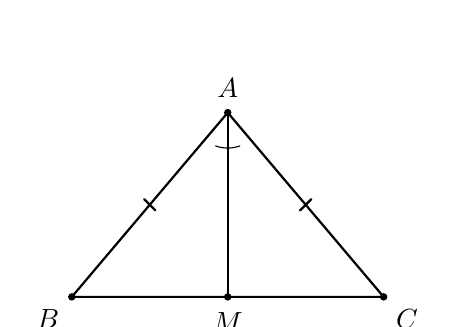
\begin{tikzpicture}[scale=0.9, line cap=round, line join=round]
  \coordinate (A) at (0,2.6);
  \coordinate (B) at (-2.2,0);
  \coordinate (C) at (2.2,0);
  \coordinate (M) at (0,0);
  \draw[thick] (B) -- (A) -- (C) -- cycle;
  \draw[thick] (A) -- (M);
  \fill (A) circle (1.5pt) node[above=2pt] {$A$};
  \fill (B) circle (1.5pt) node[below left=1pt] {$B$};
  \fill (C) circle (1.5pt) node[below right=1pt] {$C$};
  \fill (M) circle (1.5pt) node[below=2pt] {$M$};
  \draw[thick] ($(B)!0.5!(A)+(-0.08,0.08)$) -- ($(B)!0.5!(A)+(0.08,-0.08)$);
  \draw[thick] ($(C)!0.5!(A)+(-0.08,-0.08)$) -- ($(C)!0.5!(A)+(0.08,0.08)$);
  \draw (A) ++(250:0.5) arc (250:270:0.5);
  \draw (A) ++(270:0.5) arc (270:290:0.5);
\end{tikzpicture}
}
\end{ex}
\vspace{1.5mm}

\begin{ex}
Cho $A = \dfrac{1}{2^2} + \dfrac{1}{3^2} + \dfrac{1}{4^2} + \dots + \dfrac{1}{100^2}$. Chứng minh rằng $A < 1$.
\end{ex}
\vspace{1.5mm}


\begin{center}
\rule{4cm}{0.4pt}\\
\textit{--- HẾT ---}
\end{center}
\end{document}
